\newpage
\section{Xây dựng hệ thống}

Với yêu cầu của bài toán, ta cần xây dựng hệ thống cấp phát cho các doanh nghiệp, và hệ thống tra cứu thông tin nội dung cho người có nhu cầu tra cứu.\\

\begin{figure}[ht]
    \centering
    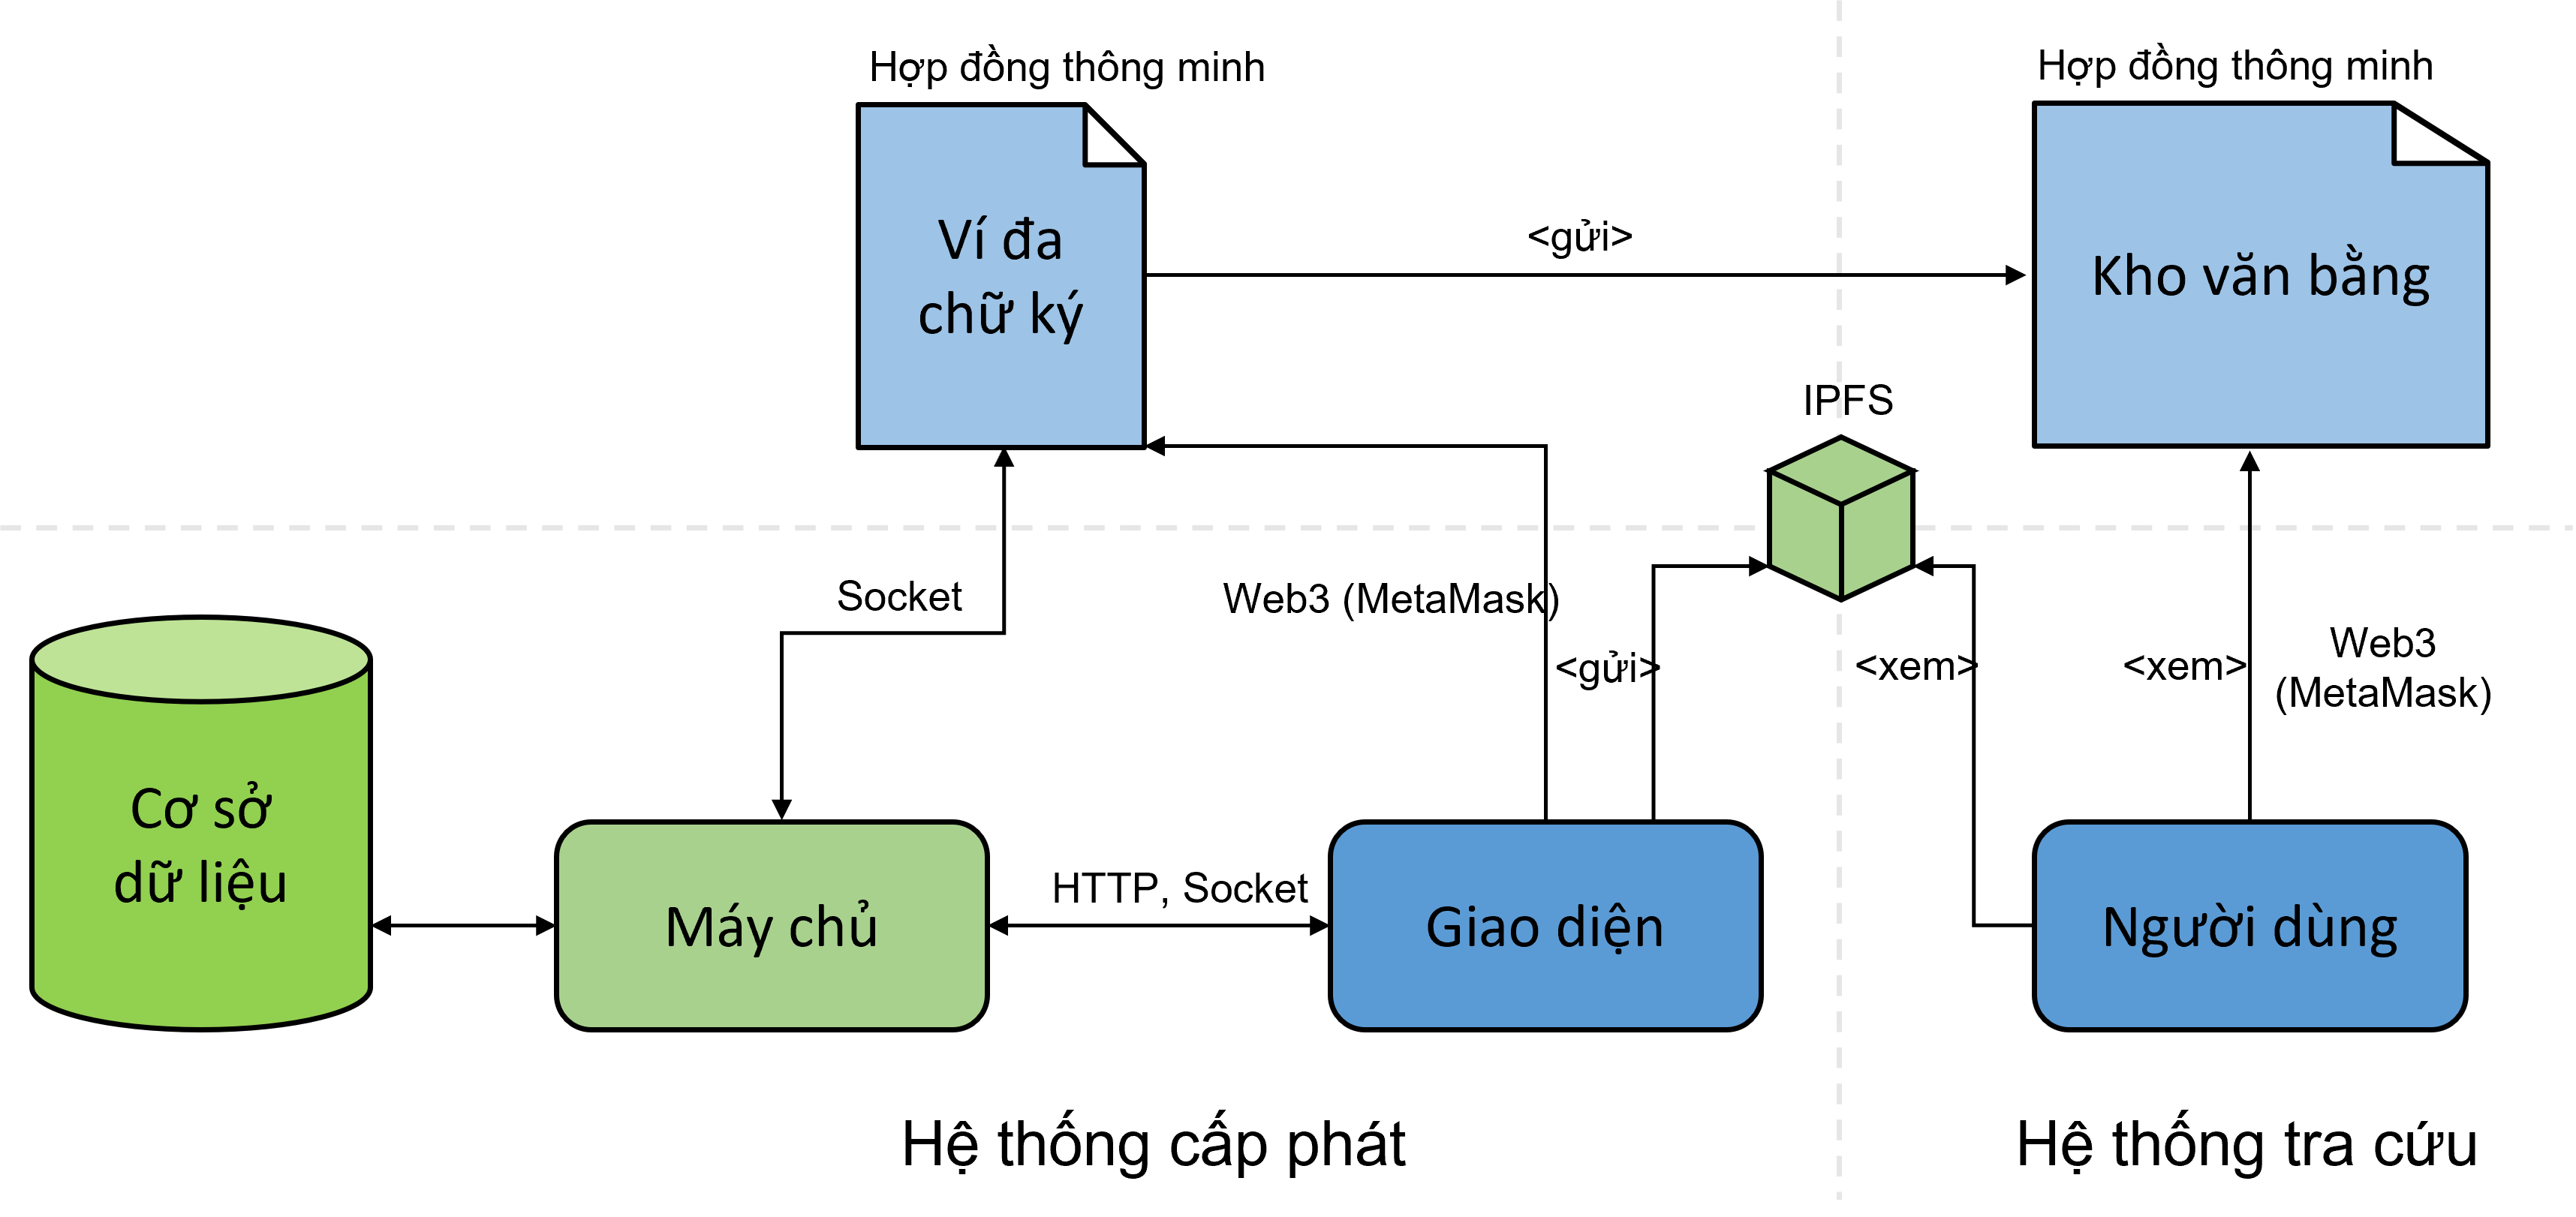
\includegraphics[width=400px]{anh/giai-phap/tong-quan-he-thong.png}
    \caption{Sơ đồ tổng quan các hệ thống và mạng chuỗi khối}
    \label{images/system-overview}
\end{figure}

Những hệ thống này sẽ tương tác với các hợp đồng thông minh trên mạng chuỗi khối, bao gồm \textit{Kho nội dung} và \textit{Ví đa chữ ký}. Trong bài báo cáo này, em xin phép tập trung trình bày về phần thiết kế các hợp đồng thông minh được triển khai cùng hệ thống.


\subsection{Kho nội dung}
\textit{Kho nội dung} là một hợp đồng thông minh nắm giữ thông tin các nội dung được lưu trữ trên mạng chuỗi khối. Thông tin được tổ chức theo cấu trúc dạng cây, mỗi mã số nội dung trên mạng chuỗi khối sẽ tương ứng với các thông tin liên quan đến nội dung đã được cấp phát.\\

Để lưu trữ nội dung trên mạng chuỗi khối, các cơ sở cấp phát cần sử dụng một địa chỉ ví để tương tác với hợp đồng thông minh được triển khai trên mạng đó. Mỗi cơ sở phát hành nội dung sẽ có một địa chỉ ví xác định, là chữ ký đại diện cho cơ sở cấp phát nội dung đó.\\

\begin{figure}[!ht]
    \centering
    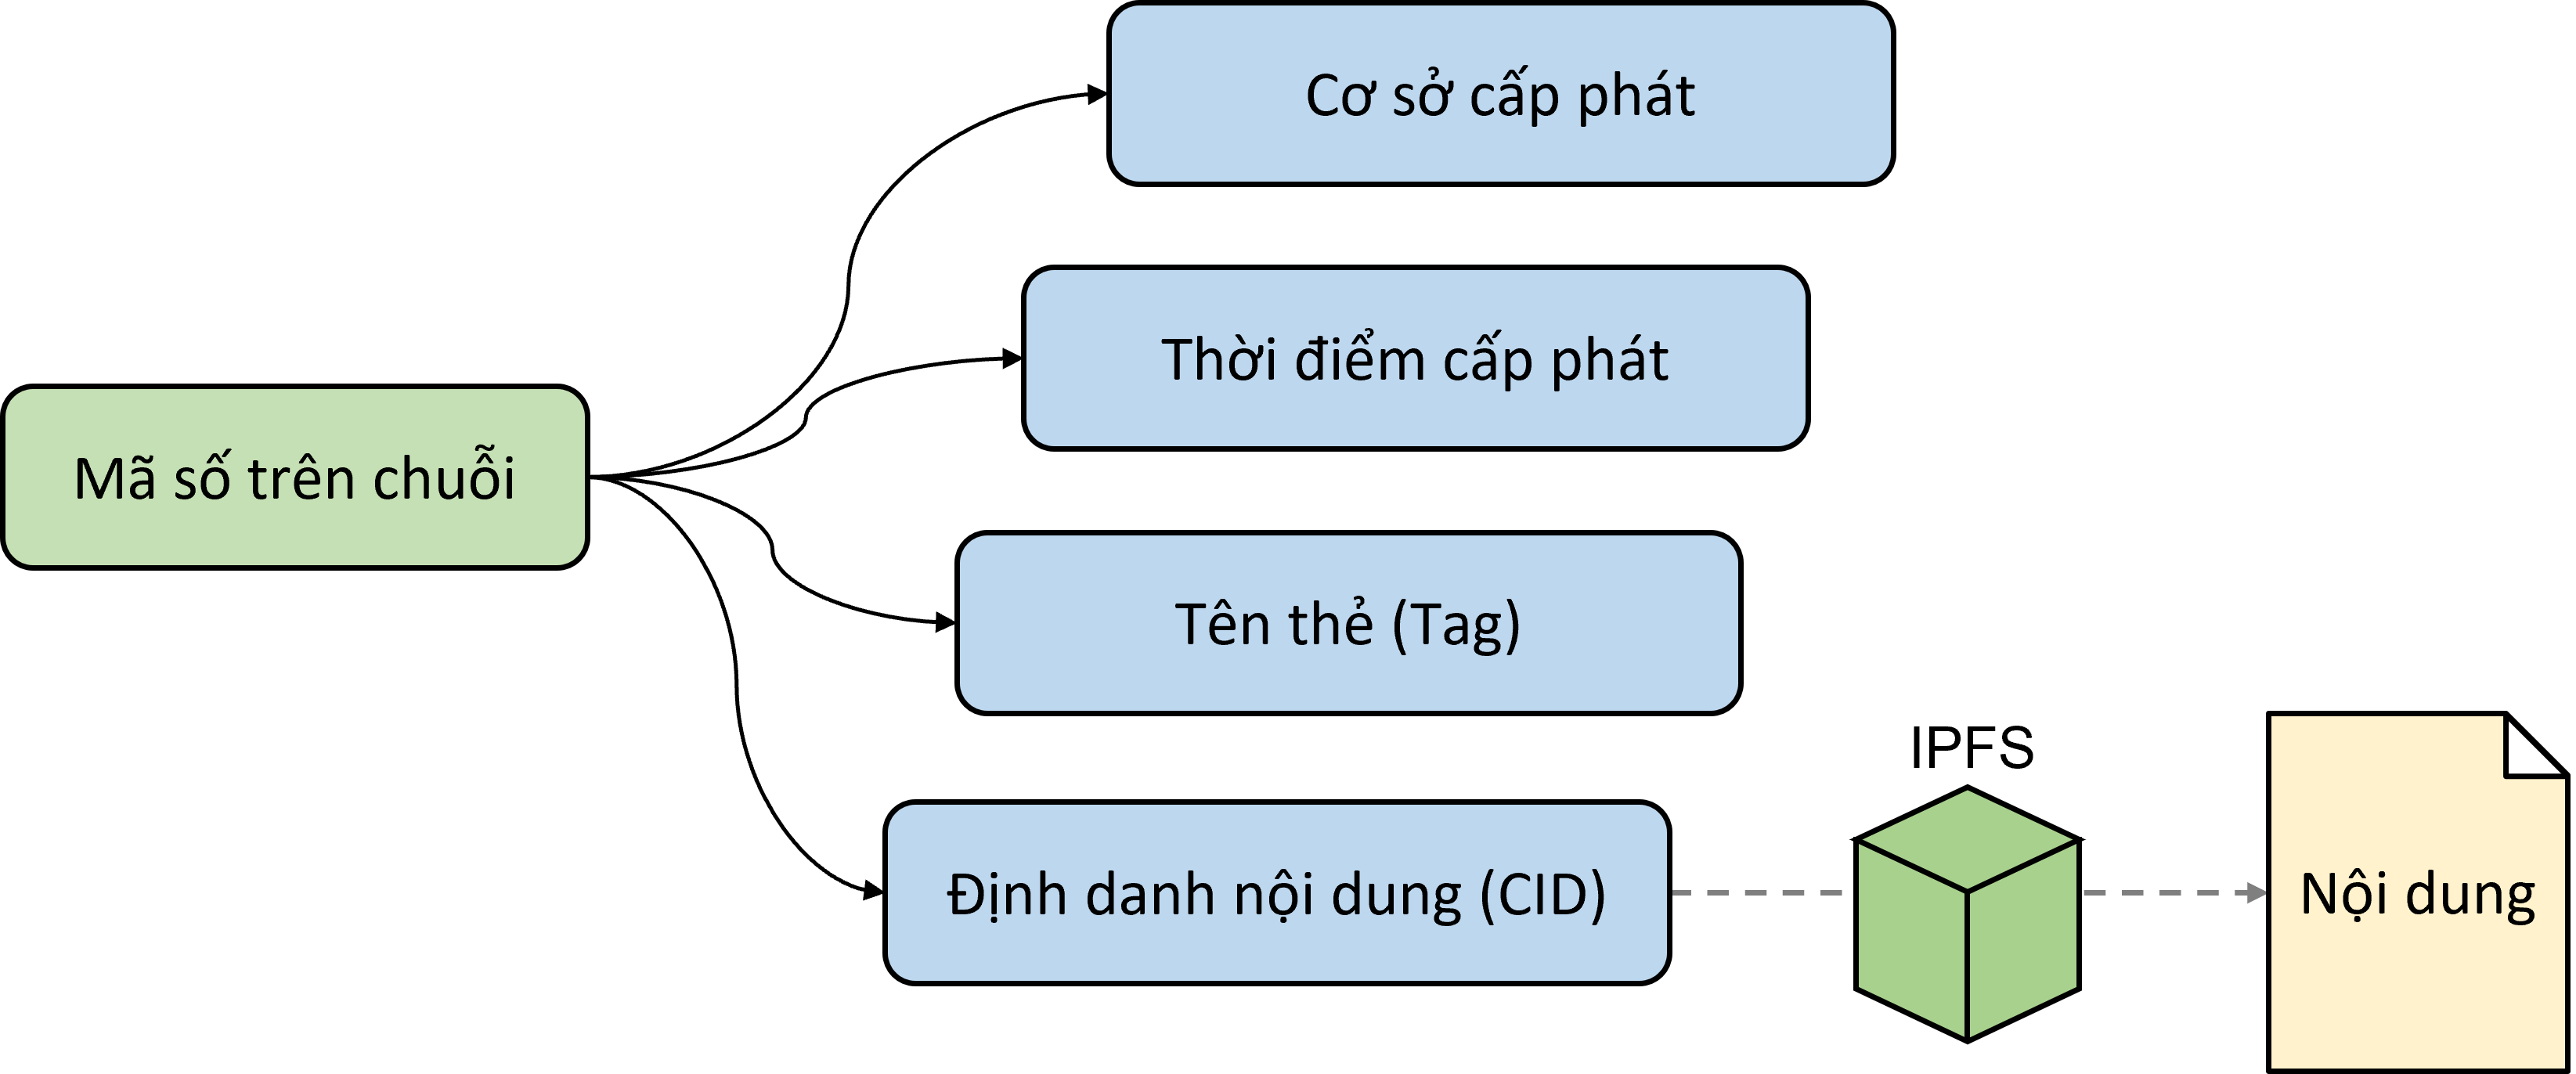
\includegraphics[width=400px]{anh/giai-phap/cau-truc-du-lieu.png}
    \caption{Cấu trúc lưu trữ thông tin trong \textit{kho nội dung}}
\end{figure}

\textit{Kho nội dung} cung cấp một số chức năng liên quan đến lưu thông tin, tra cứu thông tin nội dung. Cụ thể, ba chức năng hiện có ở đây là:
\begin{itemize}
    \item Lưu thông tin nội dung
    \item Xem thông tin nội dung
    \item Khoá nội dung
\end{itemize}

Đối với việc \textit{lưu thông tin}, địa chỉ ví của cơ sở (hay người) gửi yêu cầu lưu thông tin nội dung sẽ được lấy làm \textit{Cơ sở cấp phát}, và thông tin đi kèm sẽ được sử dụng làm \textit{Tên thẻ} cho nội dung. Như vậy, sẽ không có tình huống một cơ sở cấp phát phát hành nội dung với địa chỉ của cơ sở khác, trường hợp nhầm lẫn do vô ý hoặc có chủ đích không thể xảy ra.\\

Để \textit{xem thông tin}, người tra cứu chỉ cần cung cấp mã số nội dung đã được cấp phát. Những thông tin được hợp đồng thông minh trả về bao gồm cả định danh nội dung trên mạng IPFS, hệ thống tra cứu sẽ tự động lấy nội dung nội dung (bao gồm cả phụ lục nội dung) dựa trên định danh này.\\

Đối với trường hợp nội dung đã được cấp phát nhưng thông tin bị sai hoặc không phù hợp, phía cơ sở cấp phát nội dung có thể lựa chọn \textit{khoá nội dung} lại. Người tra cứu không thể \textit{xem thông tin} đối với những nội dung đã bị khoá.

\subsection{Ví đa chữ ký}
\textit{Ví đa chữ ký} là một hợp đồng thông minh với mục đích tăng tính bảo mật cho quá trình tương tác thay đổi thông tin nội dung trên chuỗi khối.\\

Với việc "đẩy" thông tin nội dung lên mạng chuỗi khối một cách thông thường, mỗi cơ sở cấp phát sử dụng địa chỉ ví của một cá nhân đại diện để tương tác, hoặc lựa chọn một địa chỉ ví và sử dụng chung cho cá nhân trong cơ sở. Điều này đảm bảo mỗi cơ sở cấp phát chỉ có một địa chỉ duy nhất. Tuy nhiên, khi nhiều cá nhân cùng dùng một địa chỉ ví, khả năng mất cắp tài sản liên kết với địa chỉ này càng lớn, đặc biệt khi nó còn được sử dụng trong các giao dịch khác có giá trị về tài chính (như địa chỉ sở hữu tiền mã hoá với giá trị cao trên các \textit{sàn giao dịch}\footnote{Exchange}, hay liên kết với các \textit{DApp} khác). Do đó, một cơ chế giúp giảm thiểu khả năng nhiều người cùng sở hữu một địa chỉ ví và có thể sử dụng địa chỉ ví để xác thực thông tin cơ sở cấp phát nội dung là vô cùng cần thiết. \textit{Ví đa chữ ký} ra đời để giải quyết vấn đề này.\\

Không giống với các \textit{hệ thống xác thực đa chữ ký}\footnote{Multi-signature authentication system} khi ít nhiều phụ thuộc vào các cơ chế xác thực phức tạp, \textit{ví đa chữ ký} sử dụng các tính năng, lợi thế của hợp đồng thông minh và mạng chuỗi khối. Ở \textit{ví đa chữ ký}, mỗi hành động cần thực thi (ở đây là việc cấp phát nội dung) yêu cầu một số lượng nhất định sự đồng ý từ cá nhân. Địa chỉ ví của các cá nhân này đã được thêm vào danh sách "thành viên" ngay từ khi hợp đồng thông minh này được triển khai, và họ được coi như các "cổ đông" của "doanh nghiệp" cấp phát nội dung khi có "tiếng nói" trong các "hoạt động" ở đây. Mỗi cơ sở cấp phát nội dung sử dụng một \textit{ví đa chữ ký} duy nhất, và địa chỉ của hợp đồng thông minh này đại diện cho địa chỉ ví của cả cơ sở đó. Các nội dung cần được đẩy lên \textit{kho nội dung} sẽ được một cá nhân trong cơ sở gửi lên "ví" này. Các thành viên khác trong cơ sở có thể xem thông tin các nội dung được gửi lên, và đưa ra biểu quyết "đồng ý" hay "không đồng ý" trên hợp đồng thông minh. Khi số lượng sự đồng ý đạt ngưỡng nhất định (được thiết lập từ đầu), các nội dung đó được đẩy lên "kho", và thông tin được lưu trữ trên mạng chuỗi khối.\\

\begin{figure}[!ht]
    \centering
    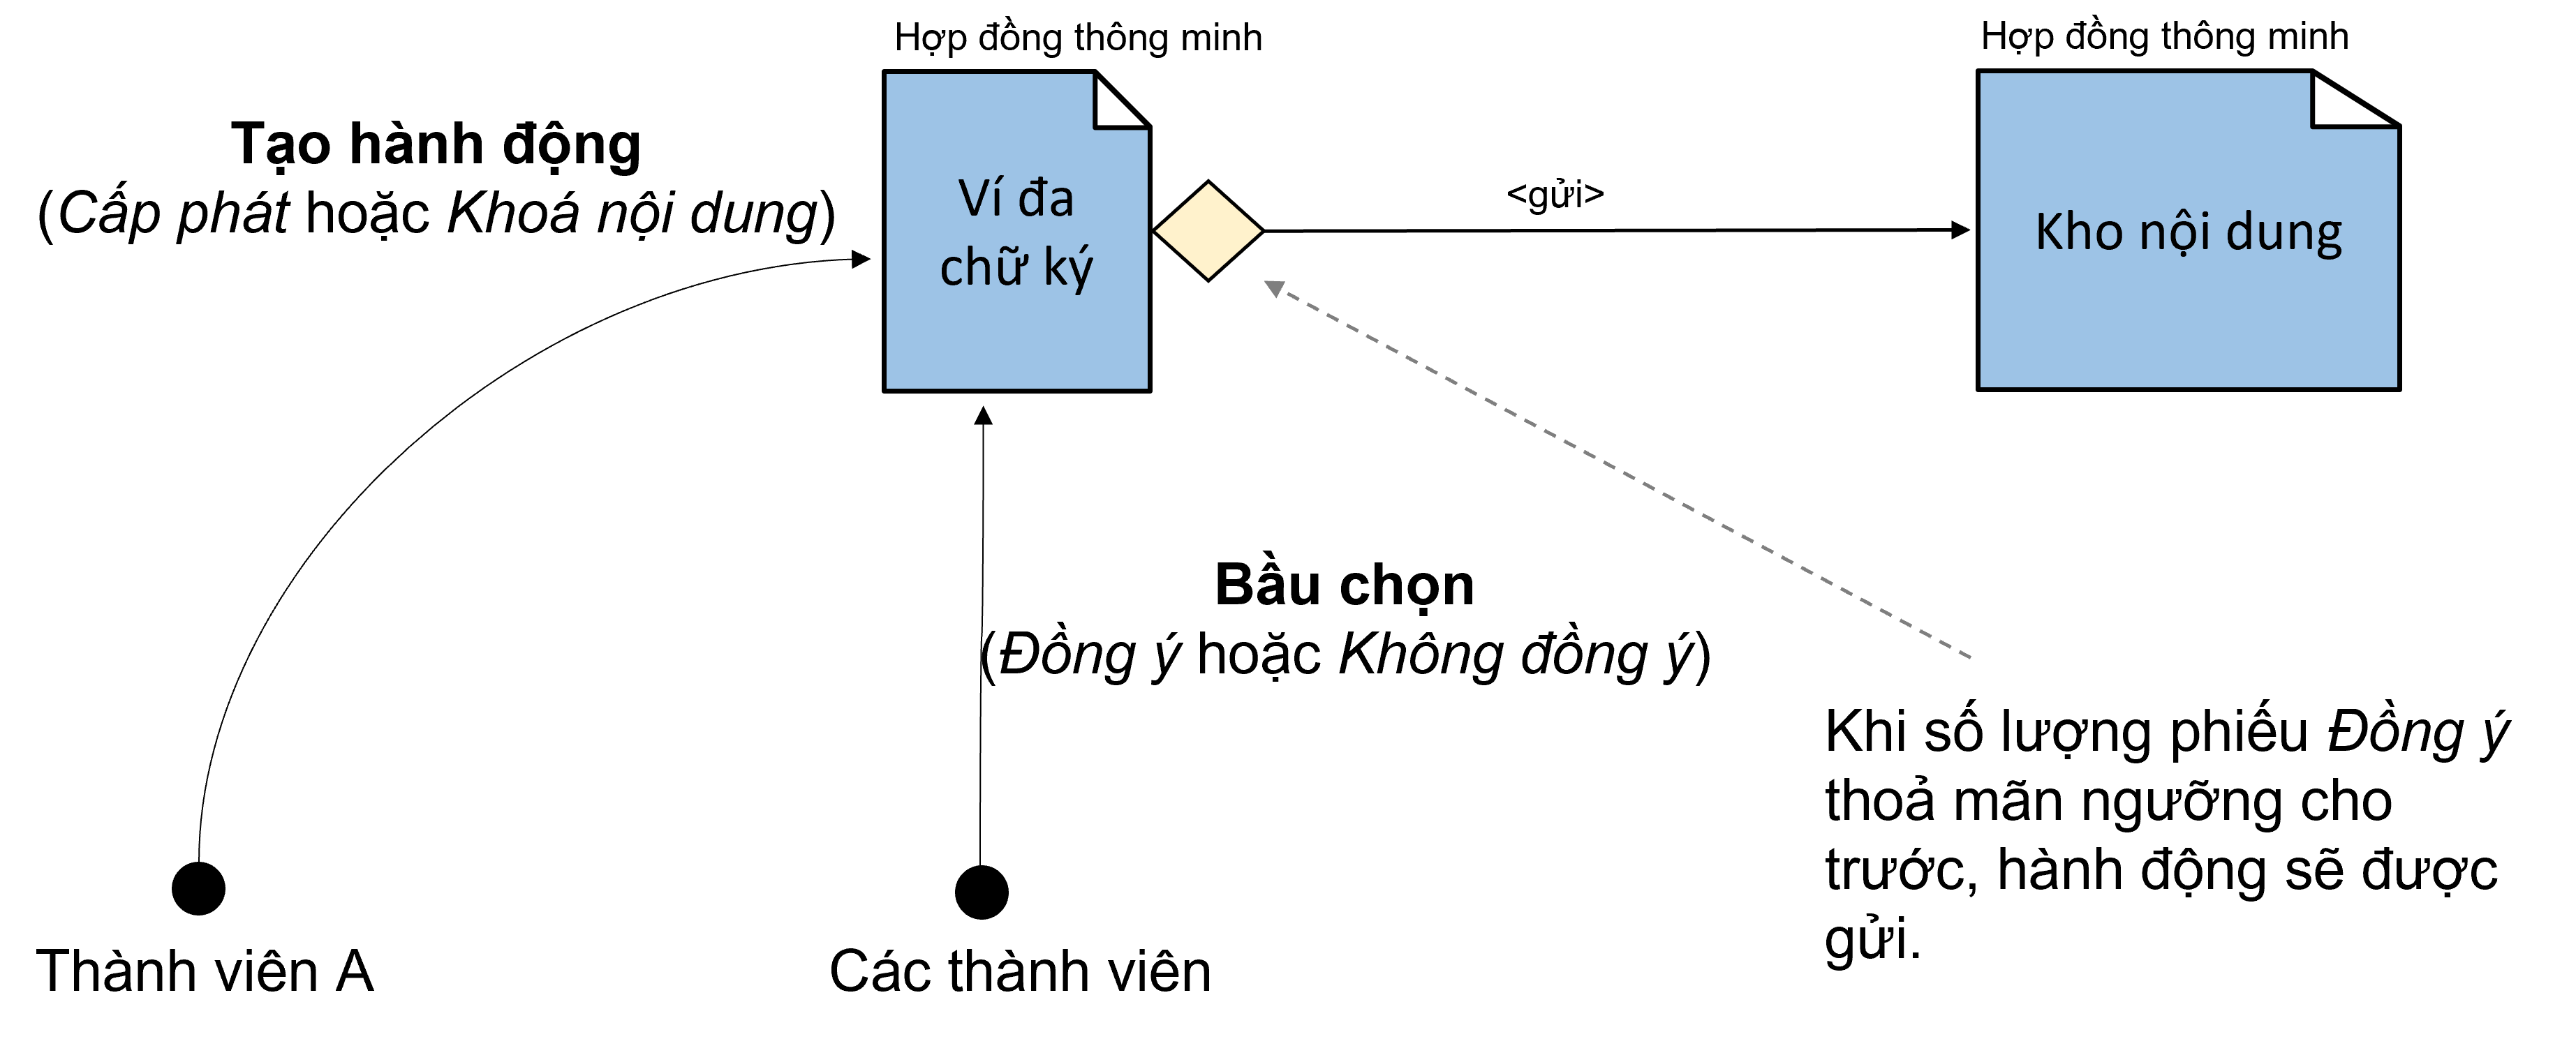
\includegraphics[width=400px]{anh/giai-phap/co-che-bau-chon.png}
    \caption{Cơ chế bầu chọn trong hệ thống}
\end{figure}

